%
% $Id: slides.tex 4228 2006-06-21 21:55:12Z jjamor $
%
%
% Compilar a .pdf con LaTeX (pdflatex)
% Es necesario instalar Beamer (paquete latex-beamer en Debian)
%

%
% Gráficos:
% Los gráficos pueden suministrarse en PNG, JPG, TIF, PDF, MPS
% Los EPS deben convertirse a PDF (usar epstopdf)
%

\documentclass{beamer}
\usetheme{Warsaw}
\usebackgroundtemplate{
\includegraphics[width=\paperwidth]{format/libresoft-bg.png}}
\usepackage[spanish]{babel}
\usepackage[utf8]{inputenc}
\usepackage{graphics}
\usepackage{amssymb} % Simbolos matematicos
\usepackage{url}

%\definecolor{libresoftgreen}{RGB}{162,190,43}
%\definecolor{libresoftblue}{RGB}{0,98,143}

%\setbeamercolor{titlelike}{bg=libresoftgreen}

%% Metadatos del PDF.
\hypersetup{
  pdftitle={Roles and organization in FLOSS communities},
  pdfauthor={F. Ortega, J.J. Amor, G. Robles, J.M Gonzalez-Barahona},
  pdfcreator={GSyC/Libresoft},
  pdfproducer=PDFLaTeX,
  pdfsubject={nn},
}
%%


\AtBeginSection[]
{
  \begin{frame}<presentation>
    \frametitle{Index}
    \tableofcontents[current]
  \end{frame}
}


\begin{document}

\title{Roles and organization in FLOSS communities}
\subtitle{Master on Free Software}
\institute{\\jfelipe@libresoft.es\\
GSyC/Libresoft}
\author{F. Ortega, J.J. Amor, G. Robles, J.M. Gonzalez Barahona}
\date{\today}

\frame{
\maketitle
\begin{center}

\includegraphics[width=6cm]{format/gsyc-urjc}
\end{center}
}


% Si el titulo o el autor se quieren acortar para los pies de p�gina
% se pueden redefinir aqu�:
%\title{Titulo corto}
%\author{Autores abreviado}


%% LICENCIA DE REDISTRIBUCION DE LAS TRANSPAS
\frame{
~
\vspace{4cm}

\begin{flushright}
{\tiny
(cc) 2007-2010 Felipe Ortega, Juanjo Amor, Gregorio Robles, Jesus M. Gonzalez Barahona. \\
Some rights reserved. This document is distributed under the Creative \\
            Commons Attribution-ShareAlike 3.0 licence, available in \\
            http://creativecommons.org/licenses/by-sa/3.0/

%  Este documento (o uno muy similar) está disponible en \\
%  \url{http://gsyc.escet.urjc.es/~jjamor/}
}
\end{flushright}
}
%%

%%%%%%
%Transpas separadas por \begin{frame}
%%%%%%%%%%%%%%%%%%%%%%%%\end{frame}

\section{Introduction}

\begin{frame}
\frametitle{So... volunteering means no organization?}
\begin{LARGE}  Not at all, we need roles and responsibilities!  \end{LARGE}
\begin{center}
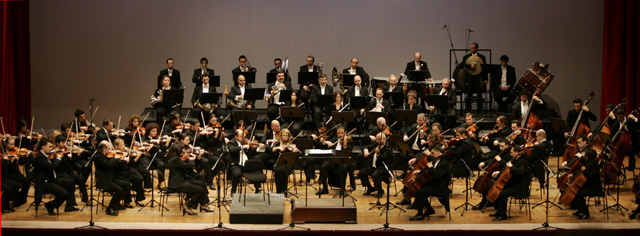
\includegraphics[width=11cm]{figs/Malta_Philharmonic_Orchestra}
\end{center}
\end{frame}

\begin{frame}
\frametitle{Overview of this unit}
\begin{itemize}
\item Identification of different roles in libre software projects.
\item Profiles and skills needed to fit in one of these roles.
\item Organization of libre software communities (\textit{``politics''}).
\end{itemize}
\end{frame}

%%%%%%%%%%%%%%%%%%%%%%%%%%%%%%%%%%%%%%%%%%%%%%%%%%%%%%%%%%%%%%

\section{Roles in FLOSS projects}

%%%%%%%%%%%%%%%%%%%%%%%%%%%%%%%%%%%%%%%%%%%%%%%%%%%%%%%%%%%%%%

\begin{frame}
\frametitle{List of possible roles in FLOSS projects}
\begin{enumerate}
 \item Developer.
 \item User.
 \item Maintainer (many sub-categories).
 \item Documentation writer.
 \item Distribution developer.
 \item Translator.
 \item Tester.
 \item Community manager.
 \item Project leader.
\end{enumerate}

\end{frame}

%%%%%%%%%%%%%%%%%%%%%%%%%%%%%%%%%%%%%%%%%%%%%%%%%%%%%%%%%%%%%%

\begin{frame}
 \frametitle{1. Developer}
 \begin{itemize}
  \item Developers work in the specification, design or development 
  (coding) of the project.
  \item Informal exchange of details and info about design: wikis, mailing lists, chats...
  \item Sometimes, they generate a document with the formal decisions about design.
  \item Control version systems for coding/developing (CVS, SVN, GIT...).
  \item They work from features requests, bugs, mailing lists and TODO lists.
 \end{itemize}

\end{frame}

%%%%%%%%%%%%%%%%%%%%%%%%%%%%%%%%%%%%%%%%%%%%%%%%%%%%%%%%%%%%%%

\begin{frame}
 \frametitle{1. Developer}
 \begin{itemize}
  \item They normally use their own IDE for the developing process.
  \begin{itemize}
   \item Specially important for developing GUIs.
  \end{itemize}
  \item But a large proportion uses editors (vim, emacs, gedit, kate...).
  \item When development is finish --> commit --> update ChangeLog.
  \item Updating the news list with new features, when a new release is closed.
 \end{itemize}

\end{frame}

%%%%%%%%%%%%%%%%%%%%%%%%%%%%%%%%%%%%%%%%%%%%%%%%%%%%%%%%%%%%%%

\begin{frame}
 \frametitle{2. User}
 \begin{itemize}
  \item Two different categories:
  \begin{itemize}
   \item Normal user.
   \begin{itemize}
    \item Do not usually compile.
    \item Use the application without many effort.
   \end{itemize}

   \item Advanced user ('techy').
   \begin{itemize}
    \item Compile the source code.
    \item Read the ChangeLog, the TODO list, etc.
   \end{itemize}

  \end{itemize}
  \item Participate in forums.
  \item Read FAQ pages.
 \end{itemize}

\end{frame}

%%%%%%%%%%%%%%%%%%%%%%%%%%%%%%%%%%%%%%%%%%%%%%%%%%%%%%%%%%%%%%

\begin{frame}
 \frametitle{3. Maintainer (many sub-categories)}
\begin{itemize}
  \item Patch manager.
  \item Translation manager.
  \item Documentation manager.
  \item Issue manager.
  \item FAQ manager.
  \item Release manager.
  \item .... manager.
\end{itemize}

\end{frame}

%%%%%%%%%%%%%%%%%%%%%%%%%%%%%%%%%%%%%%%%%%%%%%%%%%%%%%%%%%%%%%

\begin{frame}
 \frametitle{3. Maintainer (many sub-categories)}
  \begin{itemize}
   \item Patch manager.
   \begin{itemize}
    \item Look for new patches in bug tracking system.
    \item Review patches to accept or reject them.
   \end{itemize}

   \item Translation manager.
   \begin{itemize}
    \item Coordinates efforts towards internationalization 
    of the application, user manual, website, etc.
   \end{itemize}

   \item Documentation manager.
   \begin{itemize}
    \item In charge of the classically 'most tedious' task.
   \end{itemize}

  \end{itemize}

\end{frame}

%%%%%%%%%%%%%%%%%%%%%%%%%%%%%%%%%%%%%%%%%%%%%%%%%%%%%%%%%%%%%%

\begin{frame}
 \frametitle{3. Maintainer (many sub-categories)}
  \begin{itemize}
   \item Issue manager.
    \begin{itemize}
    \item Issue: Defects in software, petitions of new features, tasks.
    \item Mix between manager role, and user role.
    \end{itemize}
   \item FAQ manager.
    \begin{itemize}
     \item Create FAQ page following the first step of users in the project. Update contents adequately.
    \end{itemize}
   \item Release manager.
    \begin{itemize}
     \item Coordinate patches, new features, translations, etc. to ensure homogeneity
    \end{itemize}

  \end{itemize}

\end{frame}

%%%%%%%%%%%%%%%%%%%%%%%%%%%%%%%%%%%%%%%%%%%%%%%%%%%%%%%%%%%%%%

\begin{frame}
 \frametitle{4. Documentation writer}
 \begin{itemize}
  \item Specific role to document the application.
  \item User's manual.
  \item Man and info pages.
  \item Integration with desktop applications.
  \item Possibly create a developer's guide.
  \item Also possibly, an administrator's guide.
  \item Example: GNOME project.
  \begin{itemize}
   \item \url{http://library.gnome.org/admin/system-admin-guide/stable/index.html.en}
  \end{itemize}

 \end{itemize}

\end{frame}

%%%%%%%%%%%%%%%%%%%%%%%%%%%%%%%%%%%%%%%%%%%%%%%%%%%%%%%%%%%%%%

\begin{frame}
 \frametitle{5. Distribution developer}
 \begin{itemize}
  \item They cover the gap between distribution environment and end user environment.
  \item Support for the packaging process.
  \item Report problems to original developers.
  \item Provide integration with the installing environment (apt, yum,...).
  \item Review licenses to warrant that the application could be legally distributed.
 \end{itemize}

\end{frame}

%%%%%%%%%%%%%%%%%%%%%%%%%%%%%%%%%%%%%%%%%%%%%%%%%%%%%%%%%%%%%%

\begin{frame}
 \frametitle{6. Translator}
 \begin{itemize}
  \item They start to work in the translation of a new version when it is approved.
  \item Coordination of efforts: usually employing mailing lists.
  \item Sometimes, one per language (big projects).
  \item Messages that could be translated are frozen before the new release.
  \item No developer can change them.
  \item Translators make an extra effort to get it ready.
 \end{itemize}

\end{frame}

%%%%%%%%%%%%%%%%%%%%%%%%%%%%%%%%%%%%%%%%%%%%%%%%%%%%%%%%%%%%%%

\begin{frame}
 \frametitle{7. Tester}
 \begin{itemize}
  \item Usually, there is no specific group of testers in libre software projects.
  \begin{itemize}
   \item Everyone can act as a tester.
   \item Normal tendency: developers and advanced users.
  \end{itemize}
  \item No test plan document.
  \item Errors reported to bug tracking system.
  \item Some projects have started automatic checking processes.
 \end{itemize}

\end{frame}

%%%%%%%%%%%%%%%%%%%%%%%%%%%%%%%%%%%%%%%%%%%%%%%%%%%%%%%%%%%%%%

\begin{frame}
 \frametitle{8. Community Manager}
 \begin{itemize}
  \item They build, nurture, facilitate and expand the community around
  a FLOSS project.
  \item Frequently points of contact for new companies endorsing the project.
  \item They help to look for new sources of financing.
  \item Promote project: publicity, marketing campaigns, public image, conferences, etc.
  \item Profile:
  \begin{itemize}
   \item Very active people.
   \item They listen, they should avoid egometers.
   \item Identify teams in the community and connect them effectively.
   \item Ensure diversity, opportunities, and maintain guidelines for good conduct.
  \end{itemize}

 \end{itemize}

\end{frame}

%%%%%%%%%%%%%%%%%%%%%%%%%%%%%%%%%%%%%%%%%%%%%%%%%%%%%%%%%%%%%%

\begin{frame}
 \frametitle{9. Project Leader}
 \begin{itemize}
  \item Most relevant and influential person in the project.
  \item Meritocracy: The most active/valuable developer.
  \item Founder: The first developer or group of developers in the project.
  \item Sometimes, we find 'benevolent dictators'.
  \item Captures de essence of the motivation of the project (Torvals, Murdock, de Icaza...).
 \end{itemize}

\end{frame}


%%%%%%%%%%%%%%%%%%%%%%%%%%%%%%%%%%%%%%%%%%%%%%%%%%%%%%%%%%%%%%

\section{Organization of FLOSS and open communities}

%%%%%%%%%%%%%%%%%%%%%%%%%%%%%%%%%%%%%%%%%%%%%%%%%%%%%%%%%%%%%%

\begin{frame}
\frametitle{List of case studies}
\begin{enumerate}
 \item Apache Project (ASF).
 \item Mozilla Foundation.
 \item Wikipedia.
\end{enumerate}

\end{frame}

%%%%%%%%%%%%%%%%%%%%%%%%%%%%%%%%%%%%%%%%%%%%%%%%%%%%%%%%%%%%%%

\begin{frame}
 \frametitle{1. ASF governance}
 \begin{itemize}
  \item Users: provide feedback (bug notifications, requests...)
  \item Developers: contribute with code or documentation (active 
in mailing lists, contribute with patches, critize, etc.)
  \item Committers (around 800): developer with write access to the 
repository (has signed the CLA, can make decisions on the code subject to the PMC)
  \item Member of the PMC: developer or commiter elected by the 
Board, decides who becomes a committer, can vote on decisions that affect his subproject
  \item Member of the ASF: nominated by other members, elected by merit, ``owners'' of the ASF
 \end{itemize}

\end{frame}

%%%%%%%%%%%%%%%%%%%%%%%%%%%%%%%%%%%%%%%%%%%%%%%%%%%%%%%%%%%%%%

\begin{frame}
\frametitle{Apache's Board of Governors}

\begin{itemize}
\item Strategic, economic, legal, etc. decisions
\item Elected once a year by the members of the ASF (9 members)
\item Assigns resources to subprojects
\item Identifies the subprojects with their own committees
\end{itemize}

\end{frame}

%%%%%%%%%%%%%%%%%%%%%%%%%%%%%%%%%%%%%%%%%%%%%%%%%%%%%%%%%%%%%%

\begin{frame}
\frametitle{Apache's Officers}

\begin{itemize}
\item Elected by the Board
\item One per subproject (community)
\item One chair, president, treasurer and secretary
\item They are the executive arm of the ASF
\end{itemize}

\end{frame}

%%%%%%%%%%%%%%%%%%%%%%%%%%%%%%%%%%%%%%%%%%%%%%%%%%%%%%%%%%%%%%

\begin{frame}
\frametitle{Working Rules in Apache}

\begin{itemize}
\item Each PMC is independent and has its own rules
\item Consens, non-hierarchical, meritocratic
\item Communication: mainly mailing lists
\item Decission-taking: those who do have the power (with several limitations: lazy consens to resolve conflicts)
\item Shared philosophy
\item Incubator for new projects
\item Several horizontal committees
\end{itemize}

\end{frame}

%%%%%%%%%%%%%%%%%%%%%%%%%%%%%%%%%%%%%%%%%%%%%%%%%%%%%%%%%%%%%%

\begin{frame}
\frametitle{Project Management Committees (PMC) in Apache}

\begin{itemize}
\item At least an official of the ASF and a committer
\item The chair is elected by the Board
\item The chair defines the procedures for the daily management of a community
\item The chair decides the composition of his committee
\end{itemize}

\end{frame}

%%%%%%%%%%%%%%%%%%%%%%%%%%%%%%%%%%%%%%%%%%%%%%%%%%%%%%%%%%%%%%

\begin{frame}
\frametitle{CLAs and software grants, in Apache}

\begin{itemize}
\item Individual Contributor License Agreement: commmiters
\item Corporate CLA: companies that assign committers to the project
\item Software grant: individuals or companies that donate software to the
project (but only if they go through the incubator or are accepted by a PMC)
\end{itemize}

\end{frame}

%%%%%%%%%%%%%%%%%%%%%%%%%%%%%%%%%%%%%%%%%%%%%%%%%%%%%%%%%%%%%%

\begin{frame}
 \frametitle{2. MoFo governance}
 \begin{itemize}
  \item To have write access to the CVS, CVS Contributor Form 
(includes information about the licenses for the contribution and property of the code)
  \item Requirements: own code, permission of the employer
  \item All the code base has to be released under a project-approved license (usually MPL/LGPL/GPL)
  \item Committer acceptance process based on knowledge and merit, support from another committer
 \end{itemize}

\end{frame}

%%%%%%%%%%%%%%%%%%%%%%%%%%%%%%%%%%%%%%%%%%%%%%%%%%%%%%%%%%%%%%

\begin{frame}
 \frametitle{3. Wikipedia organization}
 \begin{itemize}
  \item Administrator.
  \item Bureaucrat.
  \item Steward.
  \item Reviewer.
  \item Oversight.
  \item Founder.
  \item Editor.
 \end{itemize}

\end{frame}

%%%%%%%%%%%%%%%%%%%%%%%%%%%%%%%%%%%%%%%%%%%%%%%%%%%%%%%%%%%%%%

\begin{frame}
 \frametitle{Exercise (I)}
 \begin{itemize}
  \item Find out information about each of the main roles in Wikipedia.
  \item Try to establish a diagram showing the connections between different roles.
  \item Can you group several roles around a specific activities?
  \item What about the Wikimedia Foundation? Can you find any governance structure?
  \end{itemize}

\end{frame}

%%%%%%%%%%%%%%%%%%%%%%%%%%%%%%%%%%%%%%%%%%%%%%%%%%%%%%%%%%%%%%

\begin{frame}
 \frametitle{Exercise (II)}
 \begin{itemize}
  \item Describe in detail the organization of the Debian community.
  \item Pay attention to the following aspects:
  \begin{itemize}
   \item Different roles.
   \item Promotion rules to access high responsibility roles.
   \item Governance rules.
  \end{itemize}

 \end{itemize}

\end{frame}

%%%%%%%%%%%%%%%%%%%%%%%%%%%%%%%%%%%%%%%%%%%%%%%%%%%%%%%%%%%%%%

\begin{frame}
 \frametitle{References}
 \begin{itemize}
 \item Karl Fogel. \textit{Producing Open Source Software: How to Run
a Successful Free Software Project}.\\
 \url{http://producingoss.com/}
 \item Jono Bacon. \textit{The Art of Community: Building the New Age
of Participation}. O'Reilly Media Inc, 2009.\\
 \url{http://www.artofcommunityonline.org}
 \item ASF governance: \url{http://apache.org/foundation/how-it-works.html}
 \item MF governance: \url{http://www.mozilla.org/about/governance.html}
 \item Wikipedia governance: \url{http://en.wikipedia.org/wiki/Wikipedia:User_access_levels}
 \end{itemize}
\end{frame}

%%%%%%%%%%%%%%%%%%%%%%%%%%%%%%%%%%%%%%%%%%%%%%%%%%%%%%%%%%%%%%

\end{document}